\section{Framework}
Once a system has been configured by an administrator using the admin portal discussed in the previous section, the BLE Location framework is available for developers to use in their Apps.  The following two sections will discuss the underlying algorithm used by the BLE Location framework, as well as the methods exposed to developers using the framework.
\subsection{Trilateration}
Trilateration is the process of using a device's known distance from three set locations to determine the point in space where that device currently is.  This algorithm is what enables the device to determine where it is relative to the set of iBeacons it currently can see.  These iBeacons broadcast information about where they are located, and the device can implicitly determine its distance from the iBeacon.  In the figure below, P1, P2, and P3 represent iBeacons, at set locations in their respective coordinate planes.  Like the iBeacons, each point has three dimensions defining its location.  In the Figure 4.2\footnote{Source: https://en.wikipedia.org/wiki/Trilateration/media/File:3spheres.svg}, all points are located on the same plane in the Z dimension for simplicity.
\begin{figure}[h]
\centering

\includegraphics[width=.55\textwidth]{images/tri.png}
\caption{Trilateration In Two Demensions}
\end{figure}

There are a variety of different ways to perform the trilateration calculations.  While Figure 4.2 shows three points sharing the same plane in the Z dimension, the underlying algorithm using the the BLE Location framework includes functionality to calculate position in three dimensions from know distances to iBeacons in three dimensions.  The algorithm and underlying code in the framework supports a Z dimension, but to keep the project within scope and to keep results accurate for proof of concept, most tests were conducted with a roughly constant plane in the Z dimension.

\begin{figure}[h]
\centering
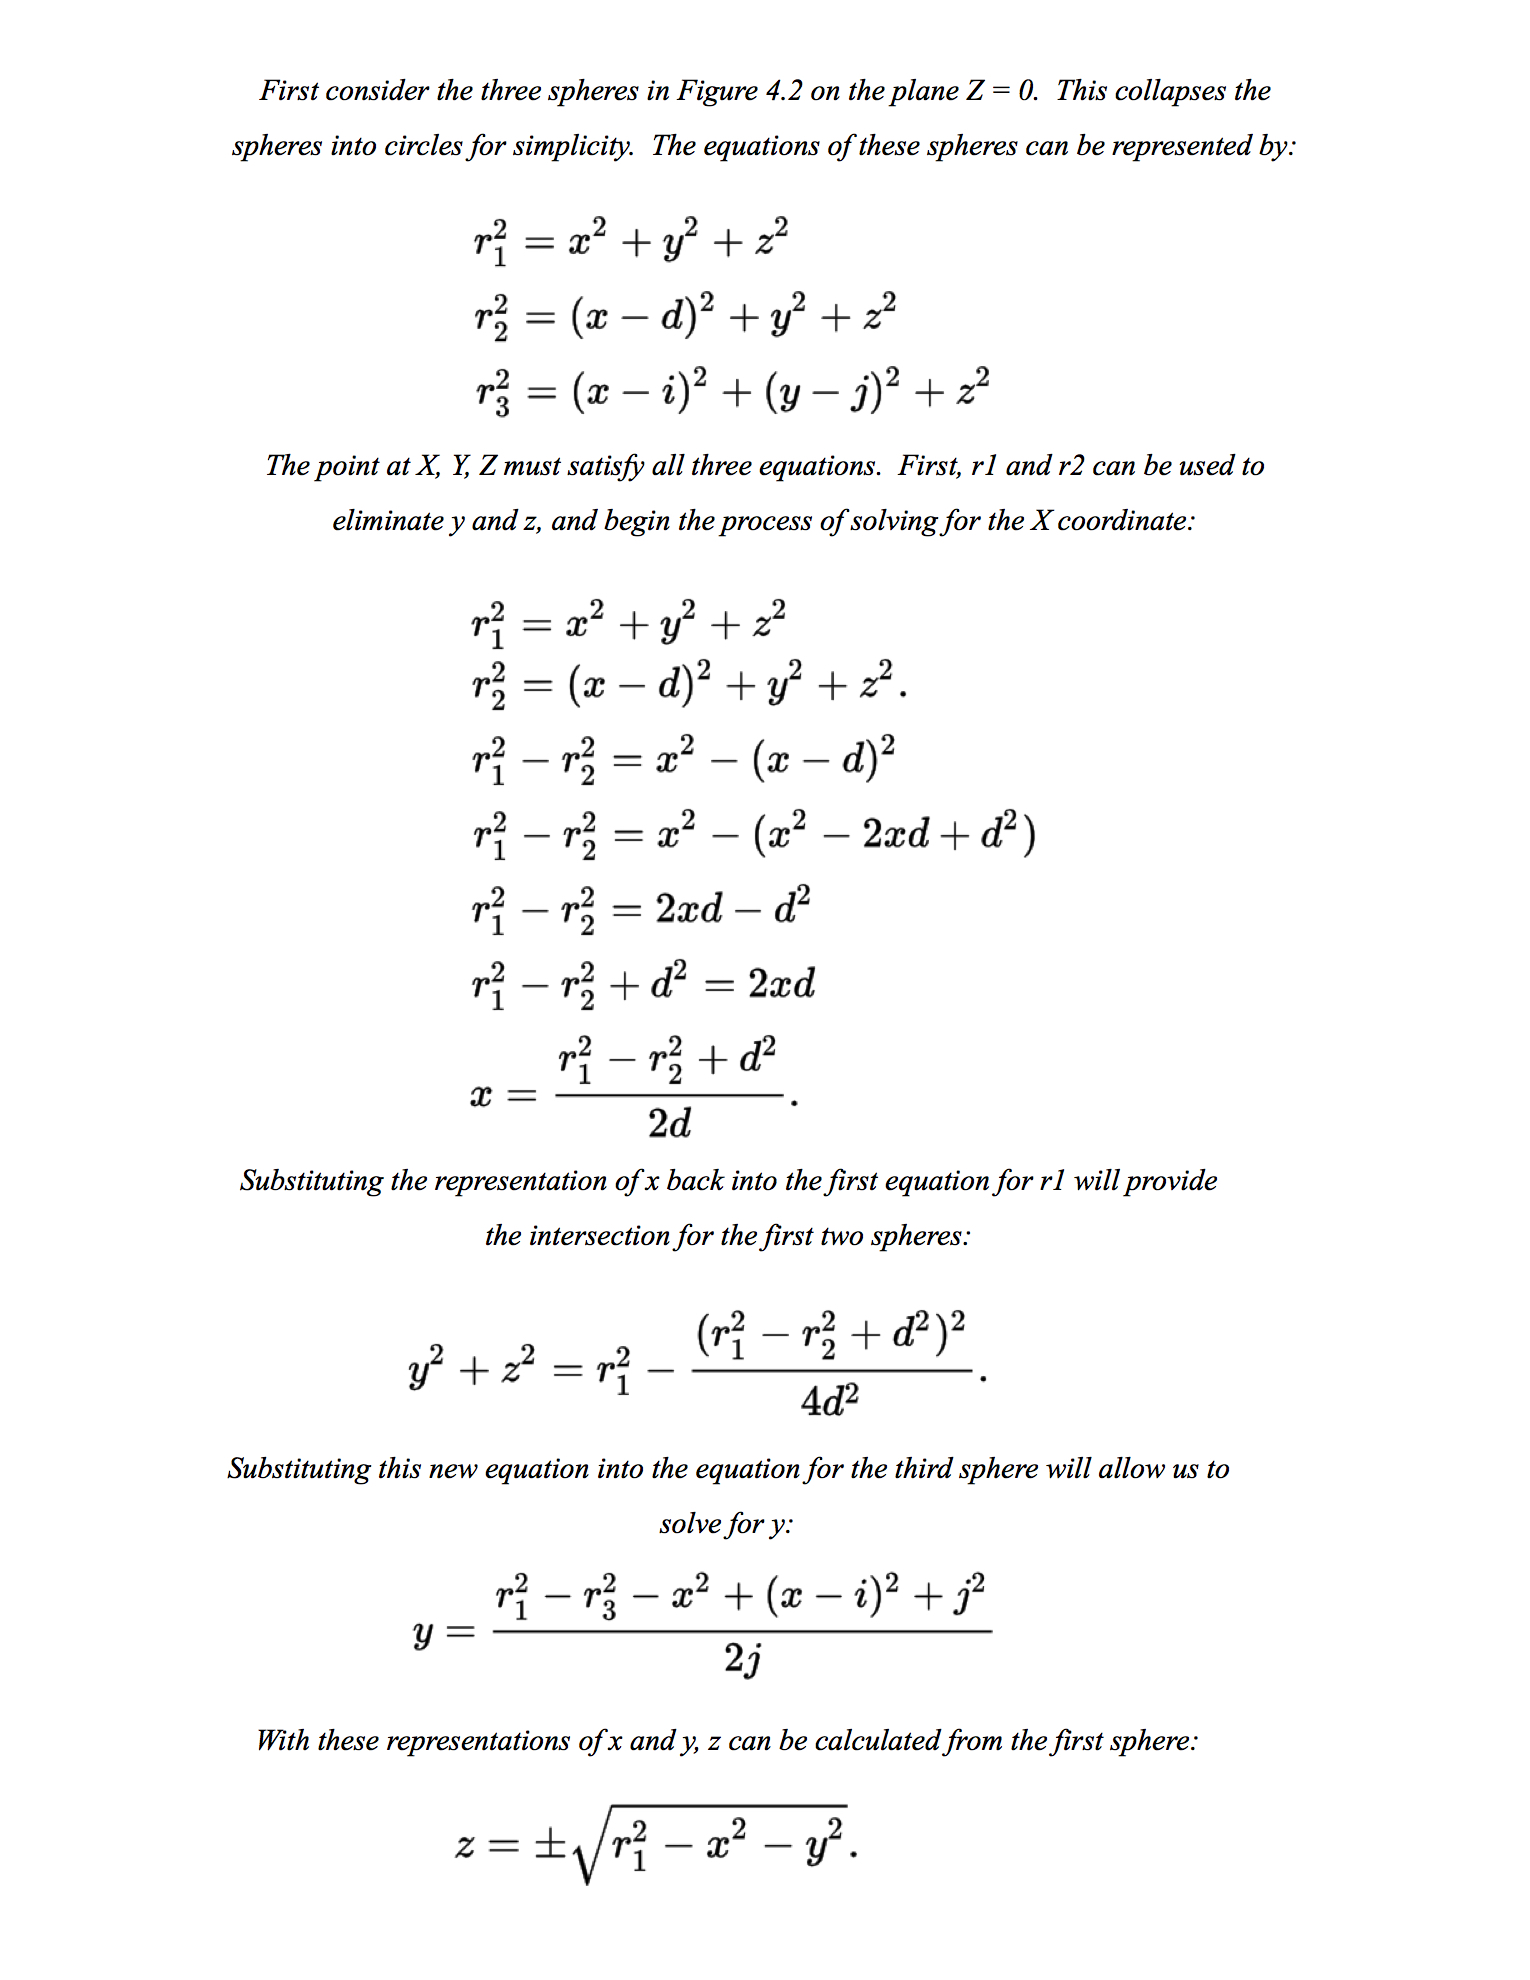
\includegraphics[width=.85\textwidth]{images/algo.jpg}
\caption{Simple Trilateration Algorithm}
\end{figure}

\subsection{BLE Location Framework for Developers}
The goal of this project was to make the BLE Location framework as simple and familiar as possible for a developer using it.  The framework follows a familiar pattern for iOS developers because it is loosely based on the delegate pattern used by the CoreLocation framework provided by Apple.  It is designed to operate on the same software layer as CoreLocation in fact, working in tandem, rather than on wrapping the whole location services package.  This allows the developer to have a higher level of control over when BLE Location is used instead of GPS or WiFi location.  The framework exposes relevant hooks with these sorts of switching operations in mind.  Figure 4.4 illustrates this context switch between GPS and BLE Location, and shows an example of how an App utilizing the framework would be able to provide an improved user experience in some cases.
\begin{figure}[h]
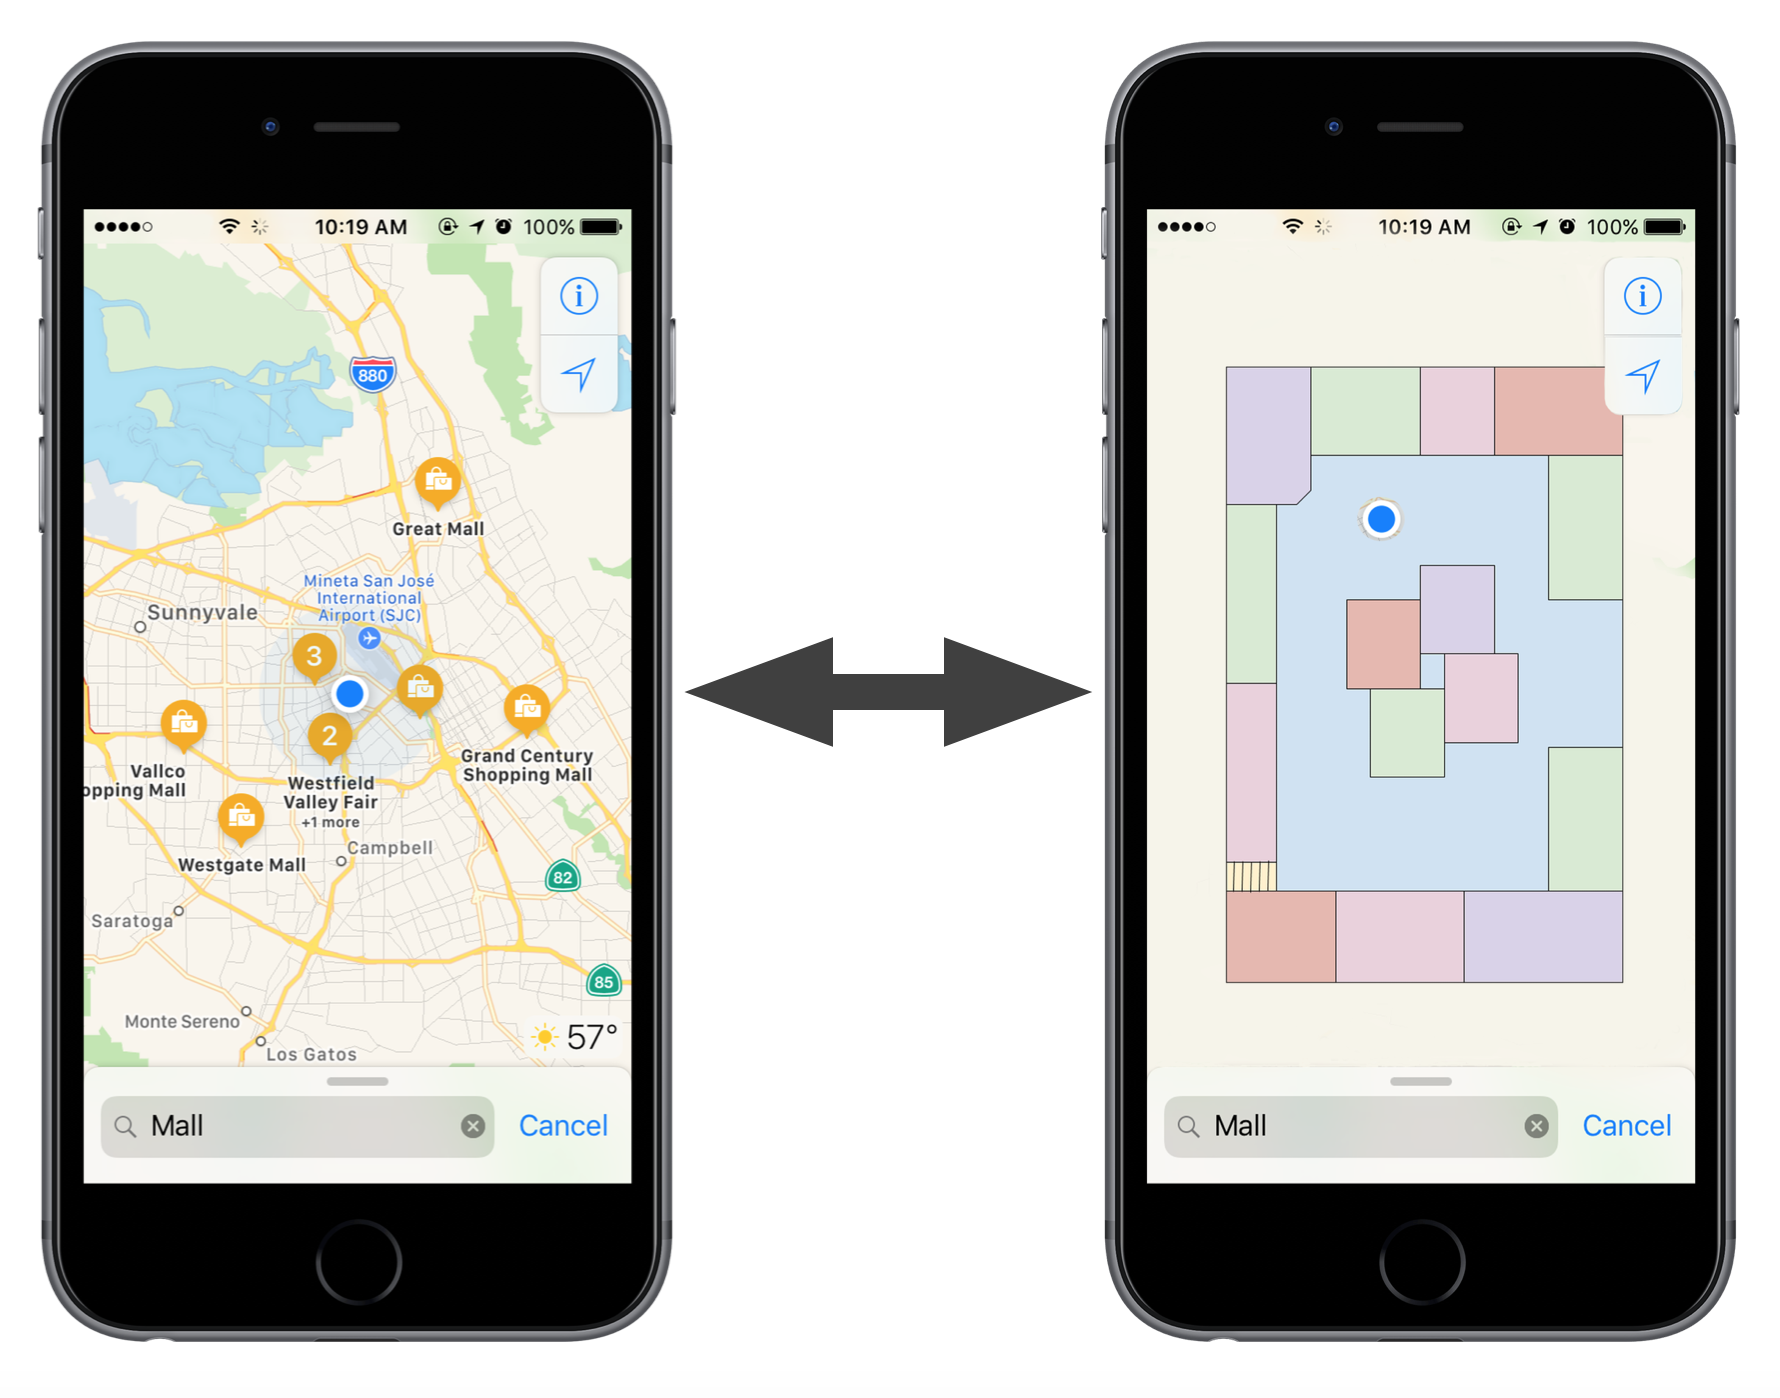
\includegraphics[width=1\textwidth]{images/compare.png}
\caption{Example location driven app using GPS (left) and BLE Location (right)}
\end{figure}

Figure X.X illustrates how the BLE Location framework could be added to a project with only a few lines of code.  After adding the framework source file to an iOS project, the developer must simply follow the basic setup illustrated below to begin integration with the BLE Location framework.  Full documentation for the BLE Location framework is available in Appendix A, however a general understanding of how it works can be gained from examining a few select parts of Figure X.X:

\begin{itemize}
\item Line 4 shows how to tell a class it must conform to the BLE Delegate Protocol.
\item Lines 12-14 show how to initialize a new BLEManger, and tell it that the current class will act as a delegate for it.
\item Line 16 shows how to begin listening for updates from the BLE Manager.
\item The functions on lines 22-37 are all examples of how to implement the functions required by the BLE Manager Delegate Protocol.
\end{itemize}

\begin{figure}[h]
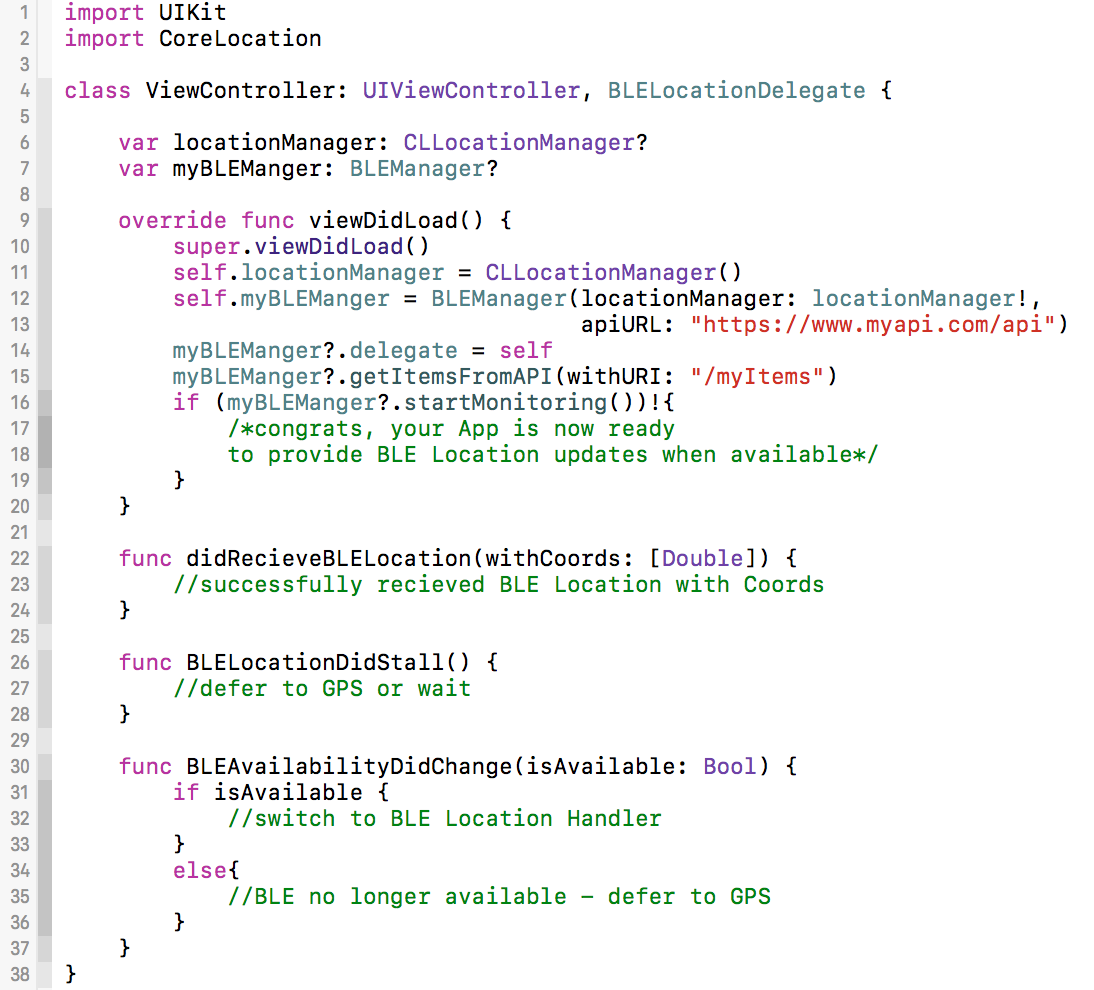
\includegraphics[width=1\textwidth]{images/code.png}
\caption{An example of how to add the BLE Location Framework to an empty iOS project}
\end{figure}

The framework is designed to work with the administrative and configuration portal documented in section 4.3.  The primary role of this admin portal is to serve information about the location and metadata of iBeacons to the framework.  The data format for the communication between the framework and portal can be found in Appendix A.  Once the framework is added to a project as seen above, and connected to the admin API as seen on line 15 of Figure X.X the framework will manage the local storage of the iBeacon data.  Once the BLE Manager has started monitoring, the different delegate protocol methods will be fired by the framework as they are triggered.  For example, once an active device comes within range of a configured group of iBeacons, the BLEAvailabilityDidChange function will fire and pass a true value.
